\documentclass[a5paper]{article}
\usepackage[a5paper, top=8mm, bottom=8mm, left=8mm, right=8mm]{geometry}

\usepackage{polyglossia}
\setdefaultlanguage[babelshorthands=true]{russian}

\usepackage{fontspec}
\setmainfont{FreeSerif}
\newfontfamily{\russianfonttt}[Scale=0.7]{DejaVuSansMono}

\usepackage[font=scriptsize]{caption}

\usepackage{amsmath}
\usepackage{amssymb,amsfonts,textcomp}
\usepackage{color}
\usepackage{array}
\usepackage{hhline}
\usepackage{cite}

\usepackage[hang,multiple]{footmisc}
\renewcommand{\footnotelayout}{\raggedright}

\PassOptionsToPackage{hyphens}{url}\usepackage[xetex,linktocpage=true,plainpages=false,pdfpagelabels=false]{hyperref}
\hypersetup{colorlinks=true, linkcolor=blue, citecolor=blue, filecolor=blue, urlcolor=blue, pdftitle=1, pdfauthor=, pdfsubject=, pdfkeywords=}

\usepackage{tabu}

\usepackage{graphicx}
\usepackage{indentfirst}
\usepackage{multirow}
\usepackage{subfig}
\usepackage{footnote}
\usepackage{minted}

\sloppy
\pagestyle{plain}

\title{Примитивы синхронизации}
\author{Юрий Литвинов\\\small{yurii.litvinov@gmail.com}}

\date{08.09.2020}

\begin{document}

\maketitle
\thispagestyle{empty}

\section{Синхронизация}

Прошлая лекция заканчивалась весьма депрессивным примером \textit{гонки} --- ситуации, когда результат работы программы зависел от случайного порядка переключения потоков планировщиком. Гонки чаще всего возникают при попытке выполнить операции с переменными, разделяемыми между потоками (если более точно, операции с общими областями памяти). При этом читать значение переменной одновременно можно безопасно, а вот запись с чтением, и тем более запись с записью, сочетаются весьма плохо. Потокам надо как-то договориться, кто в какой последовательности что делает, и, собственно, этим и занимаются механизмы синхронизации.

Лучший способ синхронизации потоков --- это сделать так, чтобы она была вообще не нужна. Бывают (и на удивление часто) такие задачи, которые элементарно распараллеливаются и решаются разными потоками от начала до конца, возможно, синхронизируясь только в конце для получения итогового ответа. Пример такой задачи (про суммирование массива) был в прошлой лекции, ещё один такой пример --- умножение матриц.

Если синхронизация всё-таки нужна, она требует поддержки либо со стороны операционной системы, либо со стороны самого процессора. Собственно, поэтому примитивы синхронизации делятся на:

\begin{itemize}
    \item User-mode-примитивы --- атомарные операции, реализующиеся на процессоре и не требующие участия планировщика. Называются User-mode, потому что операционная система о них ничего не знает и никак в процессе не участвует. Пример такой операции --- процессорная инструкция инкремента, доступная из .NET через класс Interlocked, метод \mintinline{csharp}|Interlocked.Increment()|. Она просто увеличивает значение переданной переменной на 1 атомарно, то есть операция либо проходит полностью, либо не проходит вообще.
    \item Kernel-mode-примитивы --- примитивы, управляющие тем, как поток обрабатывается планировщиком. Поскольку это требует участия операционной системы, и, соответственно, переключения в режим ядра ОС, Kernel-mode-синхронизация работает гораздо медленнее user-mode и до 1000 раз медленнее ``без синхронизации вообще''. Зато с её помощью можно делать то, что user-mode-синхронизация в принципе не может --- например, ожидание без загрузки процессора (надо понимать, что у процессора нет инструкции ``подождать'', поэтому без планировщика он вынужден работать как проклятый, исполняя программу, даже если это бесконечный цикл в духе ``событие уже произошло? а сейчас? а сейчас?''). Ещё Kernel-mode-синхронизация позволяет синхронизировать даже разные процессы.
\end{itemize}

\section{Атомарные операции}

Сегодня мы очень кратко затронем работу с user-mode-примитивами, поскольку, с одной стороны, это потребуется для понимания концепций, важных в любых многопоточных программах, но с другой стороны, подробно рассматривать мы их не будем, потому что это неизбежно приведёт к теме lock-free-программирования, которое считается чёрной магией даже среди опытных параллельных программистов\footnote{Во всех книжках, что я про это читал, пишут в самом начале, что если вам понадобилось lock-free, подумайте ещё раз. И не пользуйтесь им никогда --- а теперь, когда вы осознали эту мысль, мы вам подробно про него расскажем}. Тем не менее, выпускники матмеха должны и чёрной магией владеть, так что мы ещё вернёмся к этой теме в следующем семестре.

Итак, атомарные операции, которые не могут быть прерваны посередине и всегда либо выполняются целиком, либо не выполняются вообще, это прежде всего операции чтения и записи типов, которые целиком помещаются в машинное слово. В .NET это конкретно Boolean, Char, (S)Byte, (U)Int16, (U)Int32, (U)IntPtr, Single, все ссылочные типы (потому что ссылочные типы --- это на самом деле указатели). Это не значит, что чтение и запись в переменные этих типов совершенно безопасны и можно делать это из нескольких потоков сразу, это всего лишь значит, что вы не прострелите себе ногу ещё одним интересным образом. Положим, у нас есть значение типа Int64 изначально там было 0000. Один поток пишет туда значение 1111, другой в это же время читает. При удачном тайминге (и если предположить для простоты, что размер машинного слова у нас <<две цифры>>), читающий поток может получить значение 0011, тогда как на самом деле переменная никогда в своей жизни таким значением не обладала. Атомарность чтения и записи означает лишь, что вот такой ерунды не случится.

\section{Модель памяти}

Ещё одна очень важная вещь, связанная с атомарностью операций, это \textit{модель памяти}: логическая модель того, как ведёт себя память, кеш и ядра процессора с точки зрения прикладного многопоточного программиста. Модель памяти сильно зависит от аппаратной архитектуры процессора, потому что чем меньше ограничений она накладывает, тем быстрее может работать процессор, но тем труднее его программировать. Хорошая новость в том, что самые распространённые архитектуры --- x86 и AMD64 --- придерживаются единой модели памяти, достаточно строгой, то есть \textbf{почти} ничего плохого не делают. Тем не менее, привыкать к хорошему нельзя --- другие архитектуры, например, Itanium (IA64), SPARC с удовольствием откусят вам руку, если вы не знаете, что делаете. Казалось бы, кому какое дело до SPARC, но именно эта архитектура выбрана основой XBox360 и PlayStation 3, например. Так что если вы вдруг захотите заняться серьёзным геймдевом, вас могут ждать сюрпризы.

Концептуально модель памяти описывает то, как ядра процессора пишут в память и как они переставляют инструкции на конвейере. Насчёт записи в память концептуально дела устроены как на картинке:

\begin{tabu} {X[1 c p] X[1 c p]}
    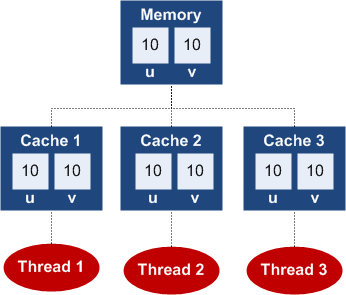
\includegraphics[width=0.35\textwidth]{volatile1.png} & 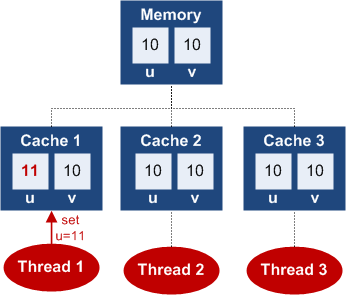
\includegraphics[width=0.35\textwidth]{volatile2.png} \\
    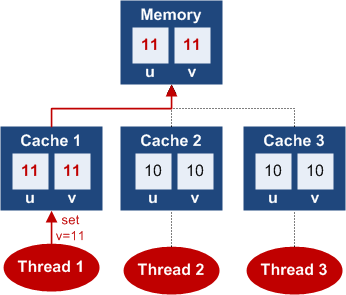
\includegraphics[width=0.35\textwidth]{volatile3.png} & 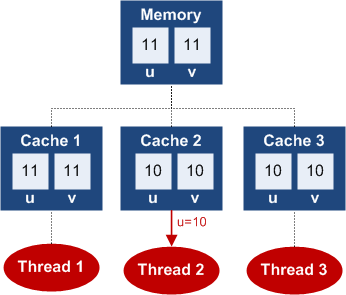
\includegraphics[width=0.35\textwidth]{volatile4.png} \\
\end{tabu}

Положим, каждый поток исполняется на своём ядре, и у них есть разделяемые переменные u и v. Изначально в них 10. Положим, первый поток пишет в u 11, сначала это значение попадает в кеш, и, вообще говоря, не обязано попасть в память. Довольно многие архитектуры не скидывают значение в память сразу, а ждут, пока значений накопится достаточно, чтобы записать их все одним запросом. Чтобы попросить ядро точно скинуть значения из кеша в память, нам потребуется специальная машинная инструкция volatile-записи, которая буквально и говорит ``запиши значение в кеш и тут же скинь кеш в память''. В нашем примере поток 1 выполняет volatile-запись значения v, сразу записывая 11 в кеш, и скидывая все значения из кеша в память. Обратите внимание, \textbf{все} значения из кеша, так что значение v, которое мирно лежало в кеше, тоже запишется. 

Теперь, положим, поток 2 хочет считать значение u из памяти. Он его читает, но читает из своего кеша, который ничего про изменения в памяти не знает, так что в качестве значения u придёт 10. Чтобы получить свежее значение, надо опять-таки воспользоваться машинной инструкцией volatile-чтения, которое имеет семантику ``обнови все имеющиеся значения в кеше и верни значение запрошенной переменной''.

На самом деле, как было сказано выше, модель памяти процессоров x86 и AMD64 умеет синхронизировать кеши, так что такие эффекты обычно не наблюдаются. ``Обычно'', потому что бывают буферы чтения-записи между кешем и регистром, они не синхронизируются. Тем не менее, прикладной программист может руководствоваться не особенностями конкретного процессора, а моделью памяти платформы. Конкретно модель памяти .NET чуть слабее, чем реализация x86: она декларирует, что все операции записи (даже обычные) исполняются как volatile, но операции чтения кеш не обновляют (то есть не volatile, даже несмотря на то, что процессор кеш обновит). Подробности см. в блоге Игоря Островского\footnote{Volatile keyword in C\# --- memory model explained, URL: \url{https://igoro.com/archive/volatile-keyword-in-c-memory-model-explained/} (дата обращения 03.09.2020)}, оттуда же без всякого согласия автора позаимствованы иллюстрации (для образовательных целей это, кажется, допустимо). Для тех, кто не боится лонгридов, очень рекомендую статью ``Memory Barriers: a Hardware View for Software Hackers''\footnote{McKenney P. E. Memory barriers: a hardware view for software hackers //Linux Technology Center, IBM Beaverton. – 2010, URL: \url{http://www.rdrop.com/users/paulmck/scalability/paper/whymb.2010.07.23a.pdf}}, там всё изложено во всех ужасных деталях.

Для тех, кто лонгриды не любит, есть простое, хотя и грубоватое правило --- все обращения к разделяемым переменным должны быть volatile. На некоторых архитектурах volatile-операции исполняются в десятки раз медленнее обычных (что не удивительно), так что более точное правило --- последняя операция записи и первая операция чтения, если у вас несколько записей подряд, или несколько чтений соответственно, должны быть volatile --- типа накидали в кеш значений, а потом скинули в память их все сразу. Если хотите ещё быстрее и лучше, читайте лонгрид.

Конкретно в .NET есть класс Volatile и его методы Volatile.Read и Volatile.Write, с, думаю, очевидной тпереь семантикой. Естьдаже ключевое слово volatile, которым можно пометить объявление поля, например, \mintinline{csharp}|private volatile int flag = 0;|. Это сделает все обращения к этой переменной volatile --- чтения будут равносильны Volatile.Read, записи --- Volatile.Write. В общем случае использование volatile может замедлить работу, но использовать его я бы рекомендовал для всех разделяемых переменных, если вы не хотите внимательно разбираться с разными эффектами. volatile, помимо упорядочения операций чтения-записи, ещё и говорит компилятору, что это разделяемая переменная и её не следует оптимизировать. Иначе может возникнуть интересный эффект, как в этом куске кода:

\begin{minted}{csharp}
static void Main(string[] args)
{
    var stop = false;
    var thread = new Thread(() => {
        stop = true;
    });

    thread.Start();

    while (!stop);

    thread.Join();

    Console.WriteLine("Done.");
}
\end{minted}

Вы думаете, что stop сразу выставится в true, мы выйдем из цикла активного ожидания и программа закончит работу? Правильно, так и будет. Но только в дебажной сборке. В релизной конфигурации программа внезапно не заканчивает работать вообще. Всё потому, что компилятор анализирует поток данных, связанный с переменной stop, видит, что она в основном потоке константна и оптимизирует обращение к ней в цикле while. Оптимизатор не такой умный, чтобы посмотреть на соседний поток, будет ли он когда-либо запущен и дойдёт ли когда-нибудь управление до изменения stop. А в дебажной конфигурации оптимизация просто не делается и всё нормально. Такие дела --- вы отлаживаетесь, у вас всё хорошо, отправляете заказчику --- всё виснет. Поправить довольно просто --- заметить, что stop разделяемая и сделать её volatile-полем (либо обернуть чтение в Volatile.Read, но это слишком умно для многих практических применений).

Вот пример правильного использования Volatile.Read и Volatile.Write, причём довольно типичный. Есть значение, которое мы считаем в одном потоке, и второй поток, который может прочитать значение, только если оно посчитано:

\begin{minted}{csharp}
private int flag = 0;
private int value = 0;

public void Thread1() {
    value = 5;
    Volatile.Write(ref flag, 1);
}

public void Thread2() {
    if (Volatile.Read(ref flag) == 1)
        Console.WriteLine(value);
}
\end{minted}

Обратите внимание, Volatile.Write послединй в серии записей, Volatile.Read первый в серии чтений.

volatile всё ещё не может спасти нас от того факта, что операция ++ не атомарна. Даже volatile-переменная, инкрементируемая одновременно из двух потоков, будет вести себя странно. Неудивительно: сначала выполняются операции чтения, которые согласованы, всё хорошо, потом прибавление в регистрах ядер, потом записи, которые тоже согласованы, всё хорошо, просто они пишут одно и то же значение. Этот вид гонки прекрасно воспроизводился бы, даже если бы кешей у ядер вообще не было. На помощь приходят атомарные операции, в частности, класс Interlocked. Рассмотрим несколько упрощённую задачу с прошлой лекции про сумму миллиона единиц:

\begin{minted}{csharp}
public int  result;

public void ThreadA()
{
    for (int i = 1; i <= 1000; i++) 
    {
        result++;
    }
}

public void ThreadB()
{
    for (int i = 1; i <= 1000; i++) 
    {
        result++; 
    }
}
\end{minted}

Как мы знаем, так она работать не будет, гонки при инкременте из разных потоков испортят нам результаты. Чтобы это поправить, заменим обычный инкремент атомарным:

\begin{minted}{csharp}
public int  result;

public void ThreadA()
{
    for (int i = 1; i <= 1000; i++) 
    {
        Interlocked.Increment(ref result);
    }
}

public void ThreadB()
{
    for (int i = 1; i <= 1000; i++) 
    {
        Interlocked.Increment(ref result); 
    }
}
\end{minted}

Теперь результат будет совершенно ожидаемым.

\section{Критические области}

Не все задачи можно решить атомарными операциями. Часто (а на самом деле, почти всегда) потокам требуется выполнять какую-то нетривиальную операцию над разделяемым ресурсом, причём так, чтобы другие потоки ему не мешали. Классический пример --- это запись в файл, но в современной практике это чаще доступ к какой-то разделяемой сложной структуре данных, например, списку или хеш-таблице. Без специальных интеллектуальных усилий (и довольно нетривиальных) попытка выполнить какие-то операции из двух потоков одновременно превращает структуру данных в кашу, поэтому проще сделать так, чтобы потоки выполняли операции строго последовательно.

Для этого в программировании используется понятие <<критическая область>> --- участок кода,  в котором одновременно может находиться только один поток. Когда поток входит в критическую область, он <<говорит>>, что она занята и все другие потоки, пытающиеся в ней попасть, пока она занята, ждут, пока она освободится. Как только поток освобождает критическую область, из ожидающих потоков выбирается (чаще всего, случайно) следующий поток и пропускается в критическую область, все остальные продолжают ждать. Поэтому критические области в параллельных программах надо использовать очень осторожно --- это то самое узкое место, у которого потоки <<толпятся>>, активно мешая друг другу. Если большая часть вычислений выполняется в критической области, то распараллеливание не принесёт радости. Визуализация происходящего представлена на рисунке~\ref{image:criticalSections}.

\begin{figure}[ht]
    \centering
        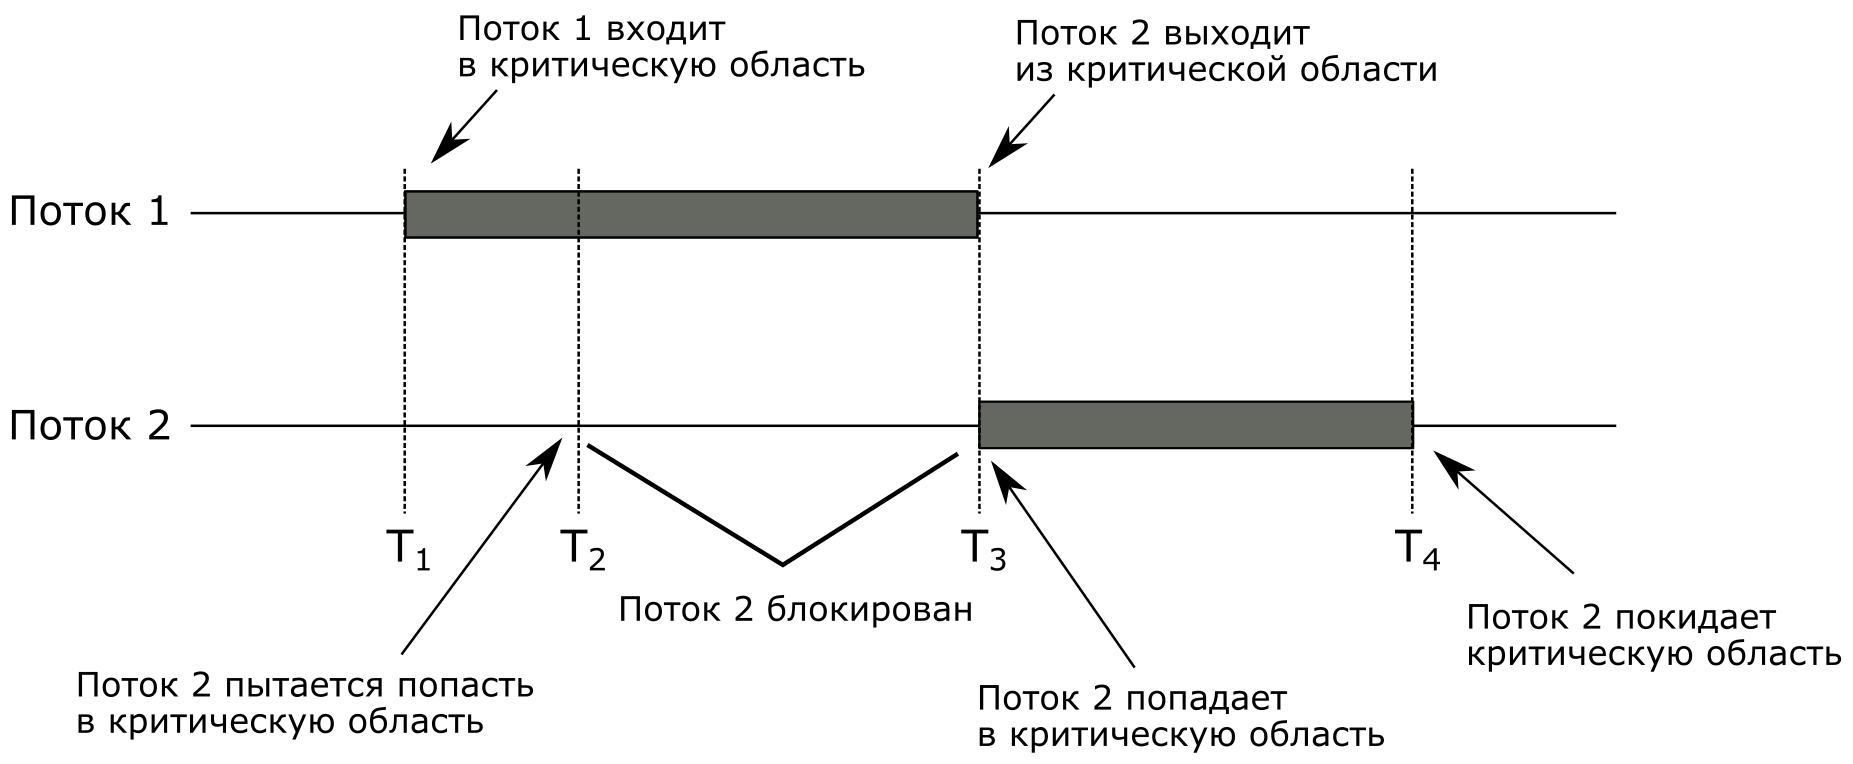
\includegraphics[width=0.8\textwidth]{criticalSections.png}
    \caption{Критические области}
    \label{image:criticalSections}
\end{figure}

\subsection{Активное ожидание}

Реализовать критические секции можно по-разному. Это можно сделать даже без участия операционной системы, правда, с тем ограничением, что без помощи планировщика потоки не могут ждать, не грузя процессор. Вот пример самой простой такой схемы:

\begin{minted}{csharp}
private int turn = 0;

void Task1()
{
    while (true)
    {
        while (turn != 0) ;
        CriticalSection();
        turn = 1;
        NonCriticalSection();
    }
}

void Task2()
{
    while (true)
    {
        while (turn != 1) ;
        CriticalSection();
        turn = 0;
        NonCriticalSection();
    }
}
\end{minted}

Есть два потока, есть код, кторый надо выполнять строго в одном потоке за раз, положим, он в методе \mintinline{csharp}|CriticalSection();|. И ещё еть некоторая часть работы, которую можно делать параллельно, она в методе \mintinline{csharp}|NonCriticalSection();|. Тогда мы заводим разделяемую переменную turn и говорим, что поток 1 может войти в критическую секцию только когда turn равен 0, а поток 2 --- только когда turn равен 1. Циклы while заставляют потоки активно ждать своей очереди, а после критической секции поток отдаёт право на посещение критической области другому потоку.

Такой подход будет работать, но обладает очевидным недостатком: ожидающий поток крутится в цикле, полностью занимая ядро процессора. Процессор-то не знает, что поток занимается ожиданием, и изо всех сил пытается исполнять его инструкции, даже если они представляют собой бесконечную последовательность условных переходов. Соответственно, растёт энергопотребление, тепловыделение, шум от системы охлаждения и, если речь идёт о мобильном устройстве, быстро разряжается аккумулятор. На самом деле, плохую параллельную программу довольно легко диагностировать --- вентилятор начинает шуметь. Ещё одна проблема --- что потоки могут работать строго по очереди, но, к счастью, это можно побороть, есть алгоритм Петерсона (который мы тут обсуждать не будем, потому что не надо использовать активное ожидание, но можете сами про него почитать).

Тем не менее, активное ожидание внезапно используется довольно часто, и этому есть рациональное объяснение --- поскольку оно не требует участия планировщика, переключение потоков может быть очень быстрым (в сотни раз быстрее, чем другими примитивами). Например, так устроен класс SemaphoreSlim (и вообще все классы с суффиксом Slim из System.Threading) стандартной библиотеки .NET --- он при попытке входа в критическую область, если она занята, пытается покрутиться в активном ожидании несколько сотен раз, и если критическая область не освобождлась, уже дёргает планировщик и честно блокируется. В случае, если критическая область короткая (что часто бывает), это позволяет сильно сэконосить на системном вызове.

Кроме того, при программировании на .NET об этом думать как-то не принято, но бывают встроенные системы, где многопоточная операционка --- большая роскошь. Там алгоритм Петерсона приходится писать вручную, потому что планировщика там просто нет.

\subsection{Проблема производителя-потребителя}

Есть несколько типичных задач, возникающих в многопоточном программировании довольно часто и требующих синхронизации. Чтобы сделать разговор о критических областях более предметным, давайте рассмотрим одну из них --- задачу производителя и потребителя (Producer-consumer problem в англоязычной литературе). Задача очень проста --- есть поток, который производит какие-то данные, есть поток, который их обрабатывает, между ними есть буфер, куда можно данные временно складировать. Производство и потребление данных может быть неравномерным, так что вполне возможны ситуации, когда буфер пустеет или переполняется, в этом случае потребитель или производитель должны временно прекратить работать, но <<проснуться>>, когда состояние буфера изменилось. Типичные применения производителя-потребителя --- поток, опрашивающий датчик и поток, делающий какие-то вычисления по показаниям (например, считающий управляющие воздействия на роботе), или сетевой драйвер и веб-сервер, который обслуживает запросы, или СУБД, которая может получать запросы из разных приложений, и т.д. Абстрактно работу производителя и потребителя в случае, когда между ними буфер из ста элементов, можно записать вот так:

\begin{minted}{csharp}
private Queue<int> buffer = new Queue<int>();

private void Producer() {
    while (true) {
        var item = ProduceItem();
        if (buffer.Count == 100)
            Sleep();
        buffer.Enqueue(item);
        if (buffer.Count == 1)
            WakeUp(Consumer);
    }
}

private void Consumer() {
    while (true) {
        if (buffer.Count == 0)
            Sleep();
        var item = buffer.Dequeue();
        if (buffer.Count == 100 - 1)
            WakeUp(Producer);
        ConsumeItem(item);
    }
}
\end{minted}

Проблема возникает в методах \mintinline{csharp}|Sleep();| и \mintinline{csharp}|WakeUp();|, их надо как-то реализовать, и в многопоточном доступе к буферу, который легко сломать, делая с ним две операции одновременно. Собственно, это можно делать с помощью разных примитивов синхронизации уровня ядра ОС.

\subsection{Семафоры}

Семафоры Дейкстры (того самого Дейкстры) --- один из самых старых, но активно использующихся до сих пор примитивов синхронизации. Семафор представляет собой целочисленный счётчик, который можно поднять (up()) и опустить (down()). down() атомарно уменьшает счётчик на 1, если он был больше нуля, или блокирует вызывающего до тех пор, пока его нельзя будет уменьшить. up() атомарно увеличивает счётчик на 1 и, если он был нулём, даёт выполнить down() одному из потоков, которые ждут своей очереди (случайному). down() обчно делается при входе в критическую секцию, up() --- при выходе, так что если счётчик изначально был равен 1, семафор даст доступ к критической секции ровно одному потоку (почему он и называется семафором, по аналогии с семафорами на железных дорогах, которые пускают только один поезд на участок пути). 

Однако счётчик изначально может быть каким угодно, и тогда в критическую секцию могут попаст не более N потоков, где N --- это начальное значение счётчика. Например, Google Drive не позволяет качать более чем десятью подключениями одновременно, поэтому, если надо скачать сотню файлов, может быть удобно создать по потоку на каждый скачиваемый файл и использовать семафор, чтобы непосредственно качало только 10 потоков. Вообще, семафор некоторые алгоритмы креативно используют как атомарную целочисленную переменную, которая блокирует вызывающий поток, если он хочет сделать её меньше нуля --- просто для того, чтобы что-то считать, например.

В случае с нашей задачей производителя-потребителя дела обстоят именно так, мы будем использовать семафоры, чтобы считать число занятых и свободных ячеек в буфере, и один \textit{бинарный} семафор, который будет охранять буфер от многопоточного доступа. Вот реализация:

\begin{minted}{csharp}
private Queue<int> buffer = new Queue<int>();
private Semaphore mutex = new Semaphore(0, 1);
private Semaphore empty = new Semaphore(100, 100);
private Semaphore full = new Semaphore(0, 100);

private void Producer()
{
    while (true)
    {
        var item = ProduceItem();
        empty.WaitOne();
        mutex.WaitOne();
        buffer.Enqueue(item);
        mutex.Release();
        full.Release();
    }
}

private void Consumer()
{
    while (true)
    {
        full.WaitOne();
        mutex.WaitOne();
        var item = buffer.Dequeue();
        mutex.Release();
        empty.Release();
        ConsumeItem(item);
    }
}
\end{minted}

Класс Semaphore в .NET принимает в конструктор начальное и максимальное значение счётчика (при попытке сделать up() на семафор с максимальным значением вызывающий блокируется). \mintinline{csharp}|WaitOne()| уменьшает значение счётчика на 1 (down() у Дейкстры), \mintinline{csharp}|Release()| увеличивает на 1 (up()). mutex ограничивает доступ к buffer и больше ничего не делает --- buffer может одновременно менять только один поток. empty в каждый момент времени равен числу свободных ячеек в буфере, full --- числу занятых. Очевидно, что одно можно получить из другого, но нам интересно не само число, а возможность блокироваться. Например, Producer блокируется на \mintinline{csharp}|empty.WaitOne()|, если в буфере нет места --- он данные произвёл, но положить их пока некуда, так что он вынужден подождать, пока потребитель хоть что-нибудь обработает. То же с потребителем --- если буфер пуст (то есть full 0), то он ждёт.

\subsection{Мьютексы}

Следующий примитив синхронизации --- мьютекс. Мьютекс (MUTual EXclusion) --- это просто бинарный семафор (то есть он пускает ровно один поток в критическую секцию). Мьютексы гораздо чаще нужны, чем семафоры (я на практике встречал семафор всего пару раз в жизни, а вот мьютексы постоянно) и проще реализуются, так что их выделяют в отдельный примитив. Мьютексы, как и семафоры, требуют участия планировщика для блокирования ожидающих потоков. В .NET мьютексы, конечно, тоже есть, вот тот же производитель-потребитель, переписанные с бинарного семаформа на настоящий мьютекс:

\begin{minted}{csharp}
private Queue<int> buffer = new Queue<int>();
private Mutex mutex = new Mutex();
private Semaphore empty = new Semaphore(100, 100);
private Semaphore full = new Semaphore(0, 100);

private void Producer()
{
    while (true)
    {
        var item = ProduceItem();
        empty.WaitOne();
        mutex.WaitOne();
        buffer.Enqueue(item);
        mutex.ReleaseMutex();
        full.Release();
    }
}

private void Consumer()
{
    while (true)
    {
        full.WaitOne();
        mutex.WaitOne();
        var item = buffer.Dequeue();
        mutex.ReleaseMutex();
        empty.Release();
        ConsumeItem(item);
    }
}
\end{minted}

По сути ничего не изменилось, \mintinline{csharp}|WaitOne()| даже называется так же, как у семафоров. Выход из критической области называется немного по-другому, \mintinline{csharp}|ReleaseMutex()|.

\subsection{Мониторы}

Следующий примитив синхронизации --- монитор Хоара --- это даже не совсем примитив, а высокоуровневая языковая конструкция, требующая поддержки не только от операционной системы, но и от компилятора. Монитор --- это набор методов (или функций), внутри которых может находиться только один поток. Монитор можно представлять себе как метод, при входе в который стоит взятие мьютекса, а в конце --- его освобождение, при этом ещё монитор будет гарантированно освобождён, если произойдёт исключение. В Java монитор --- это ключевое слово synchronized, в .NET --- конструкция lock (не совсем соответствует определению монитора, lock не метод, а ограничивает фрагмент кода, но поскольку несколько lock-ов сразу могут быть взаимоисключающими, по смыслу это монитор). Например, нашу задачу с производителем-потребителем мы могли бы реализовать совсем по-другому, перенеся всю деятельность по синхронизации в сам буфер:

\begin{minted}{csharp}
private class SynchronizedQueue {
    private Queue<int> buffer = 
        new Queue<int>();

    public void Enqueue(int item) {
        lock (buffer) {
            while (buffer.Count == 100)
                Monitor.Wait(buffer);
            buffer.Enqueue(item);
            Monitor.Pulse(buffer);
        }
    }

    public int Dequeue() {
        lock (buffer) {
            while (buffer.Count == 0)
                Monitor.Wait(buffer);
            var result = buffer.Dequeue();
            Monitor.Pulse(buffer);
            return result;
        }
    }
}

private SynchronizedQueue buffer = 
    new SynchronizedQueue();

private void Producer() {
    while (true) {
        var item = ProduceItem();
        buffer.Enqueue(item);
    }
}

private void Consumer() {
    while (true) {
        var item = buffer.Dequeue();
        ConsumeItem(item);
    }
}
\end{minted}

Класс SynchronizedQueue --- это наш новый буфер, который не только содержит элементы, но и сам блокирует вызывающего, если пуст/переполнен. lock --- это тот самый монитор, ему как параметр передаётся объект, по которому выполняется синхронизация. Как правило, это разделяемый ресурс, к которому мы хотим ограничить доступ монитором. Несколько lock-ов, у которых объект синхронизации один, взаимоисключающие, то есть поток может находиться только внутри одного из них, причём только один. Если внутрь критической секции хочет попасть второй поток, он блокируется на lock-е, пока первый из критической секции не выйдет.

\mintinline{csharp}|Monitor.Wait(buffer);| --- более интересная вещь. Оно говорит планировщику, что хоть поток и в критической секции, делать ему пока нечего, так что поток можно заблокировать, а монитор --- отдать. Теперь другой поток может войти в критическую секцию и что-то там поделать, первый поток, хоть и внутри критической секции, но спит. \mintinline{csharp}|Monitor.Pulse(buffer);| говорит, что надо пнуть один из потоков, ждущих на \mintinline{csharp}|Monitor.Wait()|, и разбудить его, как только <<пинающий поток>> отдаст монитор. В это время спящий поток пробуждается, берёт себе монитор и продолжает работу с \mintinline{csharp}|Monitor.Wait()|. При этом бывает так, что потоки будятся сами собой (<<spurious wakeup>> в англоязычной литературе), поэтому после пробуждения обязательно надо проверить условие, по которому поток был отправлен <<в спячку>>. Поэтому \mintinline{csharp}|Monitor.Wait()| обычно выполняется в цикле.

Зачем такие сложности и почему нельзя всё делать вручную через мьютексы --- потому что работа без мониторов требует большой самодисциплины и осторожности. Например, если мы посмотрим на реализацию производителя-потребителя на мьютексах и поменяем всего две строчки местами, получим дедлок:

\begin{minted}{csharp}
private Queue<int> buffer = new Queue<int>();
private Mutex mutex = new Mutex();
private Semaphore empty = new Semaphore(100, 100);
private Semaphore full = new Semaphore(0, 100);

private void Producer()
{
    while (true)
    {
        var item = ProduceItem();
        mutex.WaitOne();
        empty.WaitOne();
        buffer.Enqueue(item);
        mutex.ReleaseMutex();
        full.Release();
    }
}

private void Consumer()
{
    while (true)
    {
        full.WaitOne();
        mutex.WaitOne();
        var item = buffer.Dequeue();
        mutex.ReleaseMutex();
        empty.Release();
        ConsumeItem(item);
    }
}
\end{minted}

Мы тут переставили местами \mintinline{csharp}|empty.WaitOne();| и \mintinline{csharp}|mutex.WaitOne();| в \mintinline{csharp}|Producer();|. Казалось бы, какая разница, мы сначала берём замок на модификацию очереди, затем, если там есть свободное место, добавляем туда элемент, если нет, то ждём, пока оно появится. А оно никогда теперь не появится, потому что попытка забрать элемент из очереди в \mintinline{csharp}|Consumer();| закончится на \mintinline{csharp}|mutex.WaitOne();| --- мьютекс-то занят Producer-ом! Теперь Producer ждёт, пока в очереди появится место, а Consumer ждёт, пока ему отдадут очередь, чтобы забрать из неё элемент. Типичный дедлок. Монитор, конечно, не исключает такие фэйлы, но в силу своей высокоуровневости (и именно образа мышления, не в терминах булевых флажков, а в терминах кусков кода, в которых может быть один поток) шансов совершить ошибку сотавляет меньше. 

Кроме того, есть ещё исключения. Угадайте, что будет, если взять мьютекс и выйти из метода по исключению (которое бросил кто-то, кого мы вызываем в критической области), обойдя возврат мьютекса. Мониторы про ислючения знают и так не делают.

\subsection{lock в .NET}

Теперь более подробно о том, как lock устроен в .NET. У каждого объекта ссылочного типа в .NET (у объекта класса, строки, массива и т.п.) есть private-поле, указывающее на структуру синхронизации (грубо говоря, ту самую булевую переменную, занят монитор или нет). lock использует именно её --- когда мы входим в lock, он выставляет флажок в 1, когда выходим --- в 0. 

Так что если мы в одном и том же куске кода делаем lock на разные объекты, то это две разные критические области и они вполне могут содержать в себе два разных потока. Это может вывернуть мозг, но в этом определённо есть смысл: мы пытаемся защитить доступ к разделяемому ресурсу, и если ресурса два, то почему бы не дать двум потокам работать с ними параллельно. Хороший пример --- это метод добавления в хеш-таблицу: вот мы посчитали хеш-функцию и нашли соответствующий сегмент хеш-таблицы, в котором лежит список значений. Пока что такю функцию добавления (одну и ту же!) могут исполнять два потока одновременно, а вот добавить значение в список в два потока сразу нельзя, список сломается. Берём lock на список. Теперь добавление двух элементов с одинаковым хеш-значением будет выполняться строго последовательно, но если хеш-значения разные, то никаких проблем --- два потока меняют два разных списка и могут спокойно делать это независимо друг от друга, даже если они выполняют один и тот же код внутри lock. 

И наоборот, если lock делается на разный объект в совершенно разных кусках кода, это один монитор. Это мы видели в примере с SynchronizedQueue --- там разделяемый ресурс один (обычная очередь), а методов два. Они в одном и том же мониторе, так что в оба эти метода может одновременно попасть только один поток, и если делается \mintinline{csharp}|Enqueue();|, то \mintinline{csharp}|Dequeue();| делать уже нельзя.

И конечно же, lock умеет обрабатывать исключения. Его можно реализовать через мьютексы как try-finally, где в finally отдаётся мьютекс (кстати, в F\#, где нет ключевого слова lock, библиотечная функция lock реализована именно так). Кстати, поэтому все предыдущие примеры с семафорами и мьютексами были неправильными, они-то исключения не учитывали.

Хорошая практика --- во избежание внезапных дедлоков прятать объекты, по которым выполняется синхронизация. Может быть большой соблазн методы, которые должны быть внутри монитора, оборачивать в \mintinline{csharp}|lock(this)| (ну а что, this --- вполне себе значение ссылочного типа, оно всегда есть, всё будет работать). Однако lock на объект, на который указывает this, могут взять и извне нашего класса --- вообще в любом коде, имеющем ссылку на наш объект. Иногда ничего страшного не будет (потому что в .NET lock \textit{рекурсивный}), иногда будет дедлок --- если мы вошли в монитор и застряли в то время как другой поток вошёл в монитор, используя нас же как объект синхронизации, и застрял. Просто не делайте этого.

Часто создают просто фиктивный объект как private-поле, с единственной целью по нему синхронизироваться:
\begin{minted}{csharp}
private Object lockObject = new Object();

private void SomeMethod() {
    lock (lockObject) {
        ...
    }
}
\end{minted}

\section{Event-ы}

И напоследок, внезапно, ещё более низкоуровневый примитив синхронизации, который даже не ограничивает критическую область, а просто используется для синхронизации действий потоков. В Windows они называются \textit{Event}-ами, в Linux и в стандартной библиотеке C++ --- \textit{condition variable}-ами, в .NET --- EventWaitHandle-ами. Суть у них одна --- это булевый флажок, поддерживаемый операционной системой (точнее, планировщиком), его можно поднять и опустить. Если флажок поднят, то поток может опустить его и пройти дальше, если опущен --- то поток заблокируется, пока флажок не будет поднят. При этом поднять флажок можно в любом другом месте кода. Типичный пример использования --- создаём флажок опущенным, запускаем несколько потоков, они все блокируются на флажке, потом мы его где-то ещё поднимаем --- и все потоки проходят дальше. Типа стартуют одновременно.

Конкретно в .NET есть класс WaitHandle --- это абстракция всего, что можно ожидать, заблокировавшись средствами планировщика. От WaitHandle наследуются все примитивы синхронизации, рассмотренные выше --- семафоры (включая SemaphoreSlim, мельком упоминавшийся при рассказе об активном ожидании, пришла пора про него напомнить), мьютексы. От него же наследуется EventWaitHandle, там же определяется метод \mintinline{csharp}|WaitOne();| (и методы \mintinline{csharp}|WaitAll();|, \mintinline{csharp}|WaitAny();|, позволяющие ждать несколько событий одновременно).

От EventWaitHandle наследуются два класса, котоыре уже реально используются в коде --- AutoResetEvent и ManualResetEvent. Они очень похожи, но по-разному пропускают ждущие потоки при поднятии флага. AutoResetEvent пропускает ровно один поток и тут же опускается, остальные потоки продолжают ждать (счастливчик, как обычно, выбирается случайно). ManualResetEvent пропускает \textbf{все} ждущие потоки сразу, и опускается только тогда, когда его вручную опустят. AutoResetEvent надо использовать тогда, когда по смыслу надо разбудить только один поток, ManualResetEvent --- когда все  (например, одновременный старт потоков --- это как раз пример на ManualResetEvent).

Вот небольшой пример исползования AutoResetEvent --- вручную написанный мьютекс:

\begin{minted}{csharp}
internal class SimpleWaitLock : IDisposable {
    private readonly AutoResetEvent available;
    public SimpleWaitLock() {
        available = new AutoResetEvent(true); 
    }

    public void Enter() {
        available.WaitOne();
    }

    public void Leave() {
        available.Set();
    }

    public void Dispose() { available.Dispose(); }
}
\end{minted}

Здесь флажок создаётся поднятым, и когда первый раз делается \mintinline{csharp}|Enter();|, вызвавший поток спокойно продолжает работу. Второй поток, пытающийся сделать \mintinline{csharp}|Enter();|, видит флажок в опущенном состоянии и блокируется. И третий, и четвёртый, и т.д. Когда первый поток выходит из критической секции, он делает \mintinline{csharp}|available.Set();|, что поднимает флажок и будит ровно один поток, которому возвращается управление в \mintinline{csharp}|available.WaitOne();| и он входит в критическую секцию. Флажок тут же опускается и остальные потоки ждут своей очереди. И правда, получился замок. 

Обратите внимание, что AutoResetEvent --- IDisposable (то есть может использоваться в конструкции using), а раз он поле нашего класса, то и класс должен быть IDisposable (чтобы гарантировать удаление поля при удалении объекта класса). 

Кстати, стоит отметить, что Event-ы --- это именно булевые переменные, так что если вы сделаете \mintinline{csharp}|Set()| дважды, это вовсе не значит, что оно пропустит два потока. Может два, а может один (зависит от того, успеет отработать планировщик между двумя Set-ами или нет). Тоже способ прострелить себе ногу, будьте осторожны.

\section{Литература}

На этом про низкоуровневую многопоточность в этом курсе внезапно всё, хотя тема заслуживает ещё целого курса, и не одного. Что почитать поподробнее:

\begin{itemize}
    \item Во-первых, фундаметальную книжку Эндрю Таненбаум, Х. Бос, <<Современные операционные системы>>. По ней в основном готовилась эта лекция. Там про многопоточность не очень подробно, но зато вот алгоритм Петерсона приводится, и вообще поясняется, как оно с точки зрения ОС.
    \item Jeffrey Richter, CLR via C\# --- must read для любого .NET-программиста. Там про многопоточность вообще не очень много, но много про внутреннее устройство .NET, в частности, есть и рассказ про lock-и и WaitHandle-ы --- как они работают, как устроены, почему так. Многопоточных алгоритмов там нет, но с технической точки зрения можно много интересного узнать.
    \item Maurice Herlihy, Nir Shavit, The Art of Multiprocessor Programming --- диаметрально противоположная книжка, там очень много про многопоточные алгоритмы, но ничего про .NET. Очень рекомендую, если хотите научиться магии многопоточности по полной (но, говорят, может быть сложновата; сам почти не читал).
\end{itemize}

\end{document}
